% Name: Network topology
% Description: An office network: the internet, a firewall and router, a switch, and the machines behind it.
% Tags: network, topology, LAN, infrastructure

\usetikzlibrary{shapes.symbols}

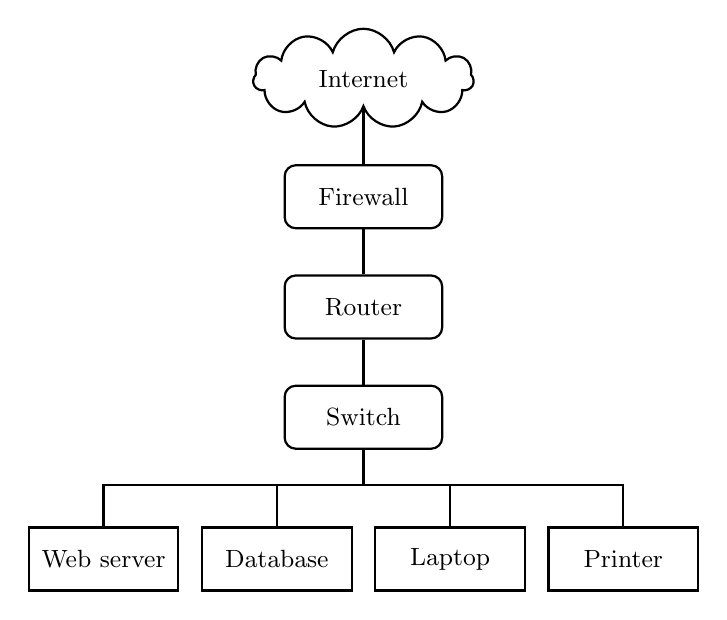
\begin{tikzpicture}[
  every node/.style={font=\small},
  device/.style={draw, thick, rounded corners, minimum width=20mm, minimum height=8mm},
  host/.style={draw, thick, minimum width=19mm, minimum height=8mm},
]
  \node[cloud, draw, thick, cloud puffs=11, aspect=2.2, minimum width=28mm] (net) at (0,4.3) {Internet};
  \node[device] (fw) at (0,2.8) {Firewall};
  \node[device] (router) at (0,1.4) {Router};
  \node[device] (switch) at (0,0) {Switch};
  \foreach \x/\name in {-3.3/Web server, -1.1/Database, 1.1/Laptop, 3.3/Printer}
    \node[host] (\name) at (\x,-1.8) {\name};

  \draw[thick] (net) -- (fw) -- (router) -- (switch);
  \foreach \name in {Web server, Database, Laptop, Printer}
    \draw[thick] (switch.south) -- ++(0,-0.45) -| (\name.north);
\end{tikzpicture}
